% **************************************************
% Document Class Definition
% **************************************************
\documentclass[%
paper=A4,                    % paper size --> A4 is default in Germany
twoside=false,                % onesite or twoside printing
openright,                    % doublepage cleaning ends up right side
parskip=full,                % spacing value / method for paragraphs
chapterprefix=true,            % prefix for chapter marks
11pt,                        % font size
headings=normal,            % size of headings
bibliography=totoc,            % include bib in toc
listof=totoc,                % include listof entries in toc
titlepage=on,                % own page for each title page
captions=tableabove,        % display table captions above the float env
draft=false,                % value for draft version
]{scrreprt}%

% **************************************************
% Debug LaTeX Information
% **************************************************
%\listfiles

% **************************************************
% Information and Commands for Reuse
% **************************************************
\newcommand{\thesisTitle}{Dự đoán giá vàng}
\newcommand{\thesisName}{Phạm Hùng Vỹ - 15521037 \\ Trần Phú Vinh- 15521020 \\ Đào Đức Huy - 15520295 \\ Phan Hữu Chí - 15520065}
\newcommand{\thesisSubject}{Báo cáo}
\newcommand{\thesisDate}{20/06/2019}
\newcommand{\thesisVersion}{1.0}

\newcommand{\teacher}{Nguyễn Công Hoan}
\newcommand{\thesisFirstReviewer}{Jane Doe}
\newcommand{\thesisFirstReviewerUniversity}{\protect{Clean Thesis Style University}}
\newcommand{\thesisFirstReviewerDepartment}{Department of Clean Thesis Style}

\newcommand{\thesisSecondReviewer}{John Doe}
\newcommand{\thesisSecondReviewerUniversity}{\protect{Clean Thesis Style University}}
\newcommand{\thesisSecondReviewerDepartment}{Department of Clean Thesis Style}

\newcommand{\thesisFirstSupervisor}{Jane Doe}
\newcommand{\thesisSecondSupervisor}{John Smith}

\newcommand{\thesisMainUniversity}{\protect{Đại học quốc gia Thành phố Hồ Chí Minh}}
\newcommand{\thesisUniversity}{\protect{Trường Đại học Công nghệ thông tin}}
\newcommand{\thesisUniversityDepartment}{Khoa công nghệ phần mềm}
\newcommand{\thesisUniversityInstitute}{Institut for Clean Thesis Dev}

\newcommand{\figureBigSize}{10cm}
\newcommand{\figureMediumSize}{10cm}
% **************************************************
% Load and Configure Packages
% **************************************************
\usepackage[utf8]{inputenc}        % defines file's character encoding
\usepackage[english]{babel} % babel system, adjust the language of the content
\usepackage{tabularx}
\usepackage{minted}
\usepackage{float}
\usepackage[                    % clean thesis style
figuresep=colon,%
sansserif=false,%
hangfigurecaption=false,%
hangsection=true,%
hangsubsection=true,%
colorize=full,%
colortheme=bluemagenta,%
bibsys=biber,%
bibfile=bib-refs,%
bibstyle=alphabetic,%
]{cleanthesis}

\hypersetup{                    % setup the hyperref-package options
pdftitle={\thesisTitle},    % 	- title (PDF meta)
pdfsubject={\thesisSubject},% 	- subject (PDF meta)
pdfauthor={\thesisName},    % 	- author (PDF meta)
plainpages=false,            % 	-
colorlinks=false,            % 	- colorize links?
pdfborder={0 0 0},            % 	-
breaklinks=true,            % 	- allow line break inside links
bookmarksnumbered=true,        %
bookmarksopen=true            %
}

% Overwrite clean thesis formating
\usepackage[T1]{fontenc}
\usepackage[sfdefault]{AlegreyaSans} %% Option 'black' gives heavier bold face
%% The 'sfdefault' option to make the base font sans serif
\renewcommand*\oldstylenums[1]{{\AlegreyaSansOsF #1}}
\usepackage[justification=centering]{caption}

% **************************************************
% Document CONTENT
% **************************************************
\begin{document}

    % --------------------------
    % rename document parts
    % --------------------------
    \renewcaptionname{english}{\figurename}{Hình.}
    \renewcaptionname{english}{\tablename}{Bảng.}
    \renewcommand{\listfigurename}{Danh sách các hình}
    \renewcommand{\contentsname}{Mục lục}

    % --------------------------
    % Front matter
    % --------------------------
    \pagenumbering{roman}            % roman page numbing (invisible for empty page style)
    \pagestyle{empty}                % no header or footers
    % !TEX root = ../chatbot-report.tex
%
% ------------------------------------  --> cover title page
\begin{titlepage}
	\pdfbookmark[0]{Cover}{Cover}
	\flushright
	\centering{
		\uppercase{ \LARGE \thesisMainUniversity} \\[6mm]
		\uppercase{ \LARGE \thesisUniversity} \\[4mm]
		\uppercase{ \LARGE \thesisUniversityDepartment} \\[4mm]
%		
\includegraphics[width=6cm]{gfx/Clean-Thesis-Logo} \\[2mm]
	}
	\hfill
	\vfill
	{\LARGE \color{ctcolortitle}\textbf{\thesisTitle} \\[10mm]}
	\rule[5pt]{\textwidth}{.4pt} \par
	\begin{minipage}[t]{.27\textwidth}
		\raggedleft
		\textit{Giảng viên hướng dẫn}
	\end{minipage}
	\hspace*{15pt}
	\begin{minipage}[t]{.65\textwidth}
		{\Large\teacher} \par
	\end{minipage} \\[5mm]
	\begin{minipage}[t]{.27\textwidth}
		\raggedleft
		\textit{Sinh viên thực hiện}
	\end{minipage}
	\hspace*{15pt}
	\begin{minipage}[t]{.65\textwidth}
		{\Large\thesisName}
	\end{minipage} \\[10mm]
	\vfill
	\vfill
	\textit{\large\thesisDate} \\
	Version: \thesisVersion
\end{titlepage}

        % INCLUDE: all titlepages
    

    \pagestyle{plain}                % display just page numbers
    %
    % !TEX root = ../chatbot-report.tex
%
\pdfbookmark[0]{Lời cảm ơn}{Thank}
\chapter*{Lời cảm ơn}
\label{sec:thank}
\vspace*{-10mm}

Nhóm chúng em hoàn thành được tốt đồ án môn học này, không thể không nói đến công lao của thầy
\teacher. Chúng em xin chân thành cảm ơn thầy đã tận tâm hướng dẫn chúng em. Bên cạnh đó, nhóm
cũng xin gửi lời cảm ơn chân thành đến các anh chị khóa trên, các bạn trong và ngoài lớp đã sẵn lòng chia sẻ tài liệu
cũng như kinh nghiệm từng trải của bản thân để nhóm chúng em học tập và tránh mắc những sai lầm, tiết kiệm được thời
gian trong quá trình thực hiện đồ án.

Tuy nhiên, do kiến thức và khả năng của chúng em còn nhiều hạn chế, do đó không tránh khỏi những thiếu sót, yếu kém.
Chúng em rất mong nhận được những ý kiến đóng góp quý báu của thầy cô và các bạn học cùng lớp để đồ án được hoàn
thiện hơn và rút ra được kinh nghiệm.
Sau cùng, chúng em xin kính chúc quý thầy cô ở Khoa Công nghệ Phần mềm, đặc biệt là thầy \teacher thật dồi dào sức khỏe để
tiếp tục thực hiện sứ mệnh cao đẹp của mình là truyền đạt kiến thức cho thế hệ mai sau.
Nhóm xin chân thành cảm ơn!
 % INCLUDE: acknowledgement
    \cleardoublepage
    %
    \setcounter{tocdepth}{3}        % define depth of toc
    \tableofcontents                % display table of contents
    \cleardoublepage


    % --------------------------
    % Body matter
    % --------------------------
    \pagenumbering{arabic}            % arabic page numbering
    \setcounter{page}{1}            % set page counter
    \pagestyle{maincontentstyle}    % fancy header and footer

    % !TEX root = ../ai-report.tex
%
\chapter{Cơ sở lý thuyết}
\label{sec:theory}

\section{Khái niệm}
\label{sec:intro:khainiem}
Dự báo đã hình thành từ đầu những năm 60 của thế kỉ 20. Khoa học dự báo với tư cách một ngành khoa học độc lập có hệ thống lí luận, phương pháp luận và phương pháp hệ riêng nhằm nâng cao tính hiệu quả của dự báo. Người ta thường nhấn mạnh rằng một phương pháp tiếp cận hiệu quả đối với dự báo là phần quan trọng trong hoạch định. Khi các nhà quản trị lên kế hoạch, trong hiện tại họ xác định hướng tương lai cho các hoạt động mà họ sẽ thực hiện. Bước đầu tiên trong hoạch định là dự báo hay là ước lượng nhu cầu tương lai cho sản phẩm hoặc dịch vụ và các nguồn lực cần thiết để sản xuất sản phẩm hoặc dịch vụ đó.
Như vậy, dự báo là một khoa học và nghệ thuật tiên đoán những sự việc sẽ xảy ra trong tương lai, trên cơ sở phân tích khoa học về các dữ liệu đã thu thập được.
Khi tiến hành dự báo ta căn cứ vào việc thu thập xử lý số liệu trong quá khứ và hiện tại để xác định xu hướng vận động của các hiện tượng trong tương lai nhờ vào một số mô hình toán học.
Dự báo có thể là một dự đoán chủ quan hoặc trực giác về tương lai. Nhưng để cho dự báo được chính xác hơn, người ta cố loại trừ những tính chủ quan của người dự báo.
Ngày nay, dự báo là một nhu cầu không thể thiếu được của mọi hoạt động kinh tế - xác hội, khoa học - kỹ thuật, được tất cả các ngành khoa học quan tâm nghiên cứu.
\section{Ý nghĩa}
\label{sec:intro:ynghia}
\begin{itemize}
    \item Dùng để dự báo các mức độ tương lai của hiện tượng, qua đó giúp các nhà quản trị doanh nghiệp chủ động trong việc đề ra các kế hoạch và các quyết định cần thiết phục vụ cho quá trình sản xuất kinh doanh, đầu tư, quảng bá, quy mô sản xuất, kênh phân phối sản phẩm, nguồn cung cấp tài chính... và chuẩn bị đầy đủ điều kiện cơ sở vật chất, kỹ thuật cho sự phát triển trong thời gian tới (kế hoạch cung cấp các yếu tố đầu vào như: lao động, nguyên vật liệu, tư liệu lao động... cũng như các yếu tố đầu ra dưới dạng sản phẩm vật chất và dịch vụ). \\
    \item Trong các doanh nghiệp nếu công tác dự báo được thực hiện một cách nghiêm túc còn tạo điều kiện nâng cao khả năng cạnh tranh trên thị trường.\\
    \item Dự báo chính xác sẽ giảm bớt mức độ rủi ro cho doanh nghiệp nói riêng và toàn bộ nền kinh tế nói chung. \\
    \item Dự báo chính xác là căn cứ để các nhà hoạch định các chính sách phát triển kinh tế văn hoá xã hội trong toàn bộ nền kinh tế quốc dân \\
    \item Nhờ có dự báo các chính sách kinh tế, các kế hoạch và chương trình phát triển kinh tế được xây dựng có cơ sở khoa học và mang lại hiệu quả kinh tế cao.\\
    \item Nhờ có dự báo thường xuyên và kịp thời, các nhà quản trị doanh nghiệp có khả năng kịp thời đưa ra những biện pháp điều chỉnh các hoạt động kinh tế của đơn vị mình nhằm thu được hiệu quả sản xuất kinh doanh cao nhất. \\
\end{itemize}
\section{Vai trò}
\label{sec:intro:vaitro}
\begin{itemize}
    \item Dự báo tạo ra lợi thế cạnh tranh \\
    \item Công tác dự báo là một bộ phận không thể thiếu trong hoạt động của các doanh nghiệp, trong từng phòng ban như: phòng Kinh doanh hoặc Marketing, phòng Sản xuất hoặc phòng Nhân sự, phòng Kế toán – tài chính. \\
\end{itemize}
\section{Các loại dự báo}
\label{sec:intro:phanloai}
Căn cứ vào độ dài thời gian dự báo: Dự báo có thể phân thành ba loại
\begin{itemize}
    \item Dự báo dài hạn: Là những dự báo có thời gian dự báo từ 5 năm trở lên. Thường dùng để dự báo những mục tiêu, chiến lược về kinh tế chính trị, khoa học kỹ thuật trong thời gian dài ở tầm vĩ mô. \\
    \item Dự báo trung hạn: Là những dự báo có thời gian dự báo từ 3 đến 5 năm. Thường phục vụ cho việc xây dựng những kế hoạch trung hạn về kinh tế văn hoá xã hội... ở tầm vi mô và vĩ mô. \\
    \item Dự báo ngắn hạn: Là những dự báo có thời gian dự báo dưới 3 năm, loại dự báo này thường dùng để dự báo hoặc lập các kế hoạch kinh tế, văn hoá, xã hội chủ yếu ở tầm vi mô và vĩ mô trong khoảng thời gian ngắn nhằm phục vụ cho công tác chỉ đạo kịp thời. \\
\end{itemize}
Cách phân loại này chỉ mang tính tương đối tuỳ thuộc vào từng loại hiện tượng để quy định khoảng cách thời gian cho phù hợp với loại hiện tượng đó: ví dụ trong dự báo kinh tế, dự báo dài hạn là những dự báo có tầm dự báo trên 5 năm, nhưng trong dự báo thời tiết, khí tượng học chỉ là một tuần. Thang thời gian đối với dự báo kinh tế dài hơn nhiều so với thang
thời gian dự báo thời tiết. Vì vậy, thang thời gian có thể đo bằng những đơn vị thích hợp ( ví dụ: quý, năm đối với dự báo kinh tế và ngày đối với dự báo dự báo thời tiết).


Dựa vào các phương pháp dự báo: Dự báo có thể chia thành 3 nhóm
\begin{itemize}
    \item Dự báo bằng phương pháp chuyên gia: Loại dự báo này được tiến hành trên cơ sở tổng hợp, xử lý ý kiến của các chuyên gia thông thạo với hiện tượng được nghiên cứu, từ đó có phương pháp xử lý thích hợp đề ra các dự đoán, các dự đoán này được cân nhắc và đánh giá chủ quan từ các chuyên gia. Phương pháp này có ưu thế trong trường hợp dự đoán những hiện tượng hay quá trình bao quát rộng, phức tạp, chịu sự chi phối của khoa học - kỹ thuật, sự thay đổi của môi trường, thời tiết, chiến tranh trong khoảng thời gian dài. Một cải tiến của phương pháp Delphi – là phương pháp dự báo dựa trên cơ sở sử dụng một tập hợp những đánh giá của một nhóm chuyên gia. Mỗi chuyên gia được hỏi ý kiến và rồi dự báo của họ được trình bày dưới dạng thống kê tóm tắt. Việc trình bày những ý kiến này được thực hiện một cách gián tiếp ( không có sự tiếp xúc trực tiếp) để tránh những sự tương tác trong nhóm nhỏ qua đó tạo nên những sai lệch nhất định trong kết quả dư báo. Sau đó người ta yêu cầu các chuyên gia duyệt xét lại những dự báo của họ trên xơ sở tóm tắt tất cả các dự báo có thể có những bổ sung thêm. \\
    \item Dự báo theo phương trình hồi quy: Theo phương pháp này, mức độ cần dự báo phải được xây dựng trên cơ sở xây dựng mô hình hồi quy, mô hình này được xây dựng phù hợp với đặc điểm và xu thế phát triển của hiện tượng nghiên cứu. Để xây dựng mô hình hồi quy, đòi hỏi phải có tài liệu về hiện tượng cần dự báo và các hiện tượng có liên quan. Loại dự báo này thường được sử dụng để dự báo trung hạn và dài hạn ở tầm vĩ mô.
    \item Dự báo dựa vào dãy số thời gian: Là dựa trên cơ sở dãy số thời gian phản ánh sự biến động của hiện tượng ở những thời gian đã qua để xác định mức độ của hiện tượng trong tương lai.
\end{itemize}

\input{content/theory/timeseries.tex}
\section{Các bước xây dựng mô hình dự đoán}
\label{sec:intro:buildmodel}
Giả sử với những dữ liêu sẵn có, ta có thể bắt đầu công việc xây dựng mô hình dự đoán qua các công đoạn sau:
\begin{enumerate}
    \item Phân tích tổng thể dữ liệu \\
    Do sự tiến bộ về các công cụ và thuật toán machine learning, nên việc xây dựng mô hình dự đoán có thể làm rất nhanh và dễ dạng. Do đó, thay vì dành phần lớn thời gian để thiết kế lại những gì đã có sẵn (mô hình dự đoán), ta dành thời gian đó cho việc quan sát sơ bộ dữ liệu để đánh giá tổng thể về độ tin cây, nhận diện các dữ liệu còn thiếu, các dữ liệu biên, các trường dữ liệu không liên quan đễn vấn đề cần giải quyết. Thời gian nay sẽ giúp chúng ta hiểu rõ hơn dữ liều mà mình đang làm việc, từ đó có cách tiếp cận đúng trong việc xây dựng mô hình dự đoán, tránh tình trạng mô hình được tạo ra dựa trên các giá trị không thực thế hay không tồn tại, ảnh hướng đến kết quả dự đoán.
    \item Xử lý sơ bộ dữ liệu (Xử lý liệu biên, dữ liệu bị thiếu) \\
    Đây được xem là phần chiếm nhiều thời gian nhất, cần những biện pháp thông minh để hoàn tất giai đoạn này. Đây là những cách để chúng ta sử lý những dữ liệu xấu.
    \begin{itemize}
	    \item Gán những biến tạm cho các giá trị còn thiếu: các giá trị còn thiếu của một  lượng thông tin có thể cho chúng ta biết nhiều điều. Bằng cách gán các giá trị tạm để mô hình dự đoán biết đó là giá trị còn thiếu có thể cho ra các kết quả chuẩn xác hơn. \\
	    \item Gán những giá trị còn thiếu bằng giá trị trung bình trong cùng một trường dữ liệu (data imputation). Đây cũng là cách phổ biến để xử lý các dữ liệu còn thiếu. \\
    \end{itemize}
    \item Xây dựng mô hình dự đoán \\
    Sử dụng các công cụ hoặc các thuật toán để xây dụng mô hình dựa trên các dữ liệu đã được xử lý. Các kỹ thuật để xây dựng mô hình dự đoán sẽ được đề cập ở phần sau, Machine Learning. \\
    \item Đánh giá sự chính xác của mô hình. \\
    Đánh giá độ chính xác của các Model dựa các công thức đã sẵn có. \\
\end{enumerate}

\textbf{Recurrent neural network} \\[0.2em]
Con người không bắt đầu suy nghĩ từ đầu mỗi giây.
Khi bạn đọc bài luận này, bạn hiểu từng từ dựa trên sự hiểu biết của bạn về các từ trước đó.
Bạn không nên ném mọi thứ đi và bắt đầu suy nghĩ lại từ đầu. Suy nghĩ của bạn
có sự lưu lại.

Mạng lưới thần kinh truyền thống có thể làm được điều này, và nó có vẻ như là một
thiếu sót lớn.
Ví dụ, hãy tưởng tượng bạn muốn phân loại loại sự kiện nào đang diễn ra tại mọi thời điểm trong phim.
Nó không rõ làm thế nào một mạng lưới thần kinh truyền thống có thể sử dụng lý lẽ của nó về các sự kiện trước đó trong phim để thông báo cho những sự kiện sau này.

Recurrent neural network giải quyết vấn đề này. Chúng là các mạng có các vòng lặp trong đó, cho phép thông tin tồn tại.
\begin{figure}[!htb]
    \center{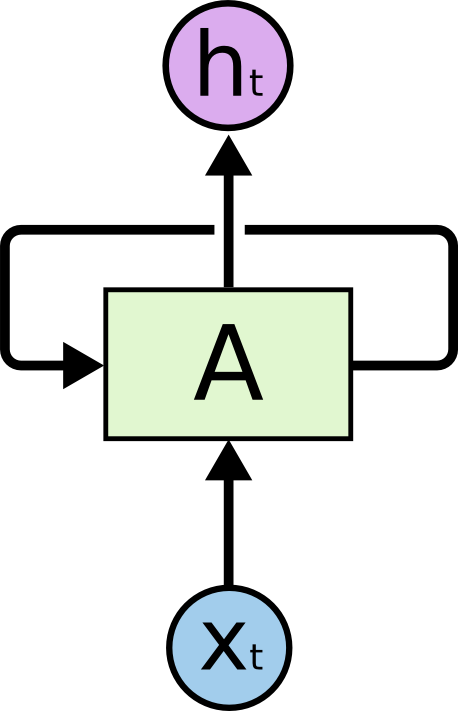
\includegraphics[width=4cm]
    {figure/model/RNN-rolled.png}}
    \caption{\label{fig:rnn-rolled} Recurrent Neural Network có vòng lặp.}
\end{figure}

Trong sơ đồ trên, một đoạn của mạng thần kinh, \(A\), xem xét một số \(x_t\) đầu vào và xuất ra một giá trị
\(h_t\).Một vòng lặp cho phép thông tin được truyền từ một bước của mạng sang bước tiếp theo.

Những vòng lặp này làm cho Recurrent neural network có vẻ như bí ẩn.
Tuy nhiên, nếu bạn suy nghĩ nhiều hơn một chút, hóa ra họ không phải là một mạng lưới thần kinh bình thường.
Recurrent neural network có thể được coi là nhiều bản sao của cùng một mạng, mỗi bản tin truyền cho một người kế nhiệm.
Xem xét những gì xảy ra nếu chúng ta bỏ vòng lặp:

\begin{figure}[!htb]
    \center{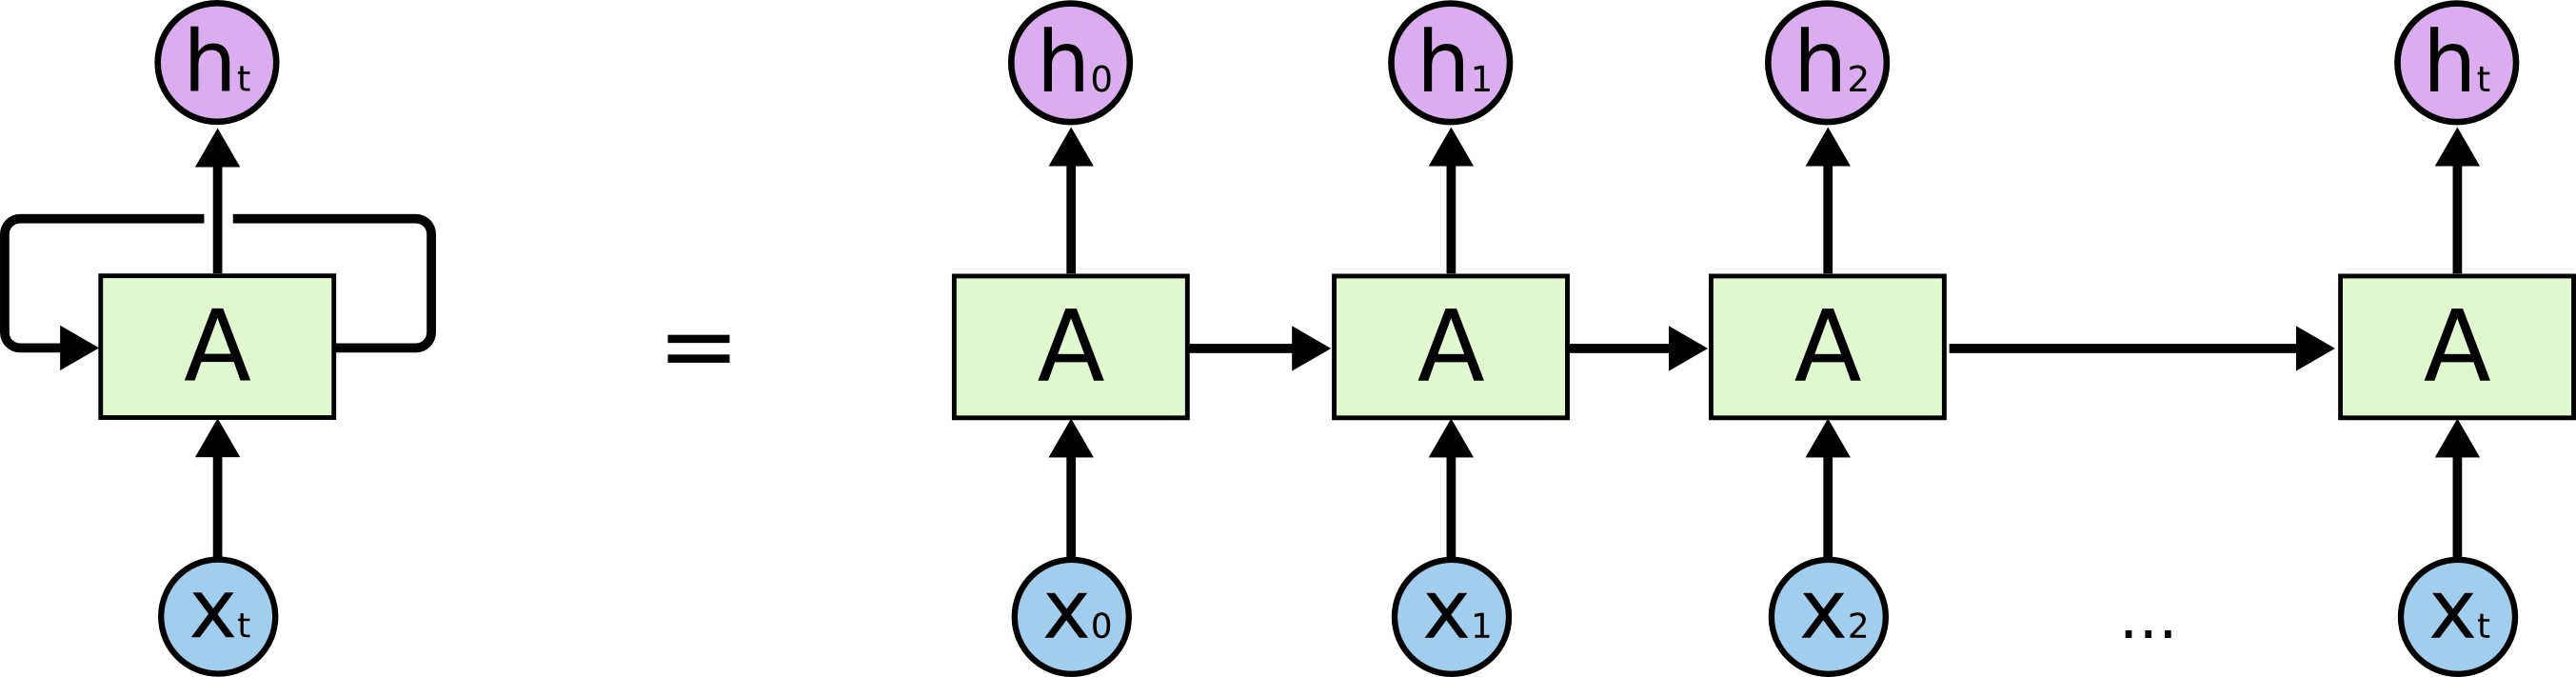
\includegraphics[width=\figureBigSize]
    {figure/model/RNN-unrolled.png}}
    \caption{\label{fig:rnn-unrolled} Recurrent Neural Network đã được trải ra.}
\end{figure}

Bản chất giống như chuỗi này cho thấy các Recurrent neural network có liên quan mật thiết đến các chuỗi và danh sách.
Nó sử dụng kiến trúc tự nhiên của mạng neuron để sử dụng cho dữ liệu đó.

Và chúng chắc chắn được sử dụng!
Trong vài năm qua, đã có những thành công đáng kinh ngạc khi áp dụng RNN cho nhiều vấn đề khác nhau: nhận dạng giọng
nói, mô hình ngôn ngữ, dịch thuật, chú thích hình ảnh.

Điều cần thiết cho những thành công này là việc sử dụng "LSTM", một loại Recurrent neural network rất đặc biệt, hoạt
động, cho nhiều tác vụ, tốt hơn nhiều so với phiên bản tiêu chuẩn. Hầu như tất cả các kết quả thú vị dựa trên các mạng thần kinh tái phát đều đạt được với chúng. Nó có những LSTM mà bài tiểu luận này sẽ khám phá.

\textbf{Vấn đề phụ thuộc xa} \\[0.2em]
Một trong những lời kêu gọi của RNN là ý tưởng rằng họ có thể kết nối thông tin trước đó với tác vụ hiện tại, chẳng
hạn như sử dụng các khung video trước đó có thể thông báo cho sự hiểu biết về khung hiện tại. Nếu RNN có thể làm điều
này, thì họ cực kỳ hữu ích. Nhưng họ có thể? Không hẳn.

Đôi khi, chúng ta chỉ cần nhìn vào thông tin gần đây để thực hiện nhiệm vụ hiện tại. Ví dụ, hãy xem xét một mô hình
ngôn ngữ đang cố gắng dự đoán từ tiếp theo dựa trên các từ trước đó. Nếu chúng ta đang cố gắng dự đoán từ cuối cùng
trong "các đám mây trên \textit{bầu trời}", thì chúng ta không cần bất kỳ bối cảnh nào nữa - đó là một điều khá rõ ràng,
từ tiếp theo sẽ là  \textit{bầu trời}. Trong những trường hợp như vậy, khi khoảng cách giữa thông tin liên quan và
địa điểm mà nó cần là nhỏ, RNN có thể học cách sử dụng thông tin trong quá khứ.

\begin{figure}[!htb]
    \center{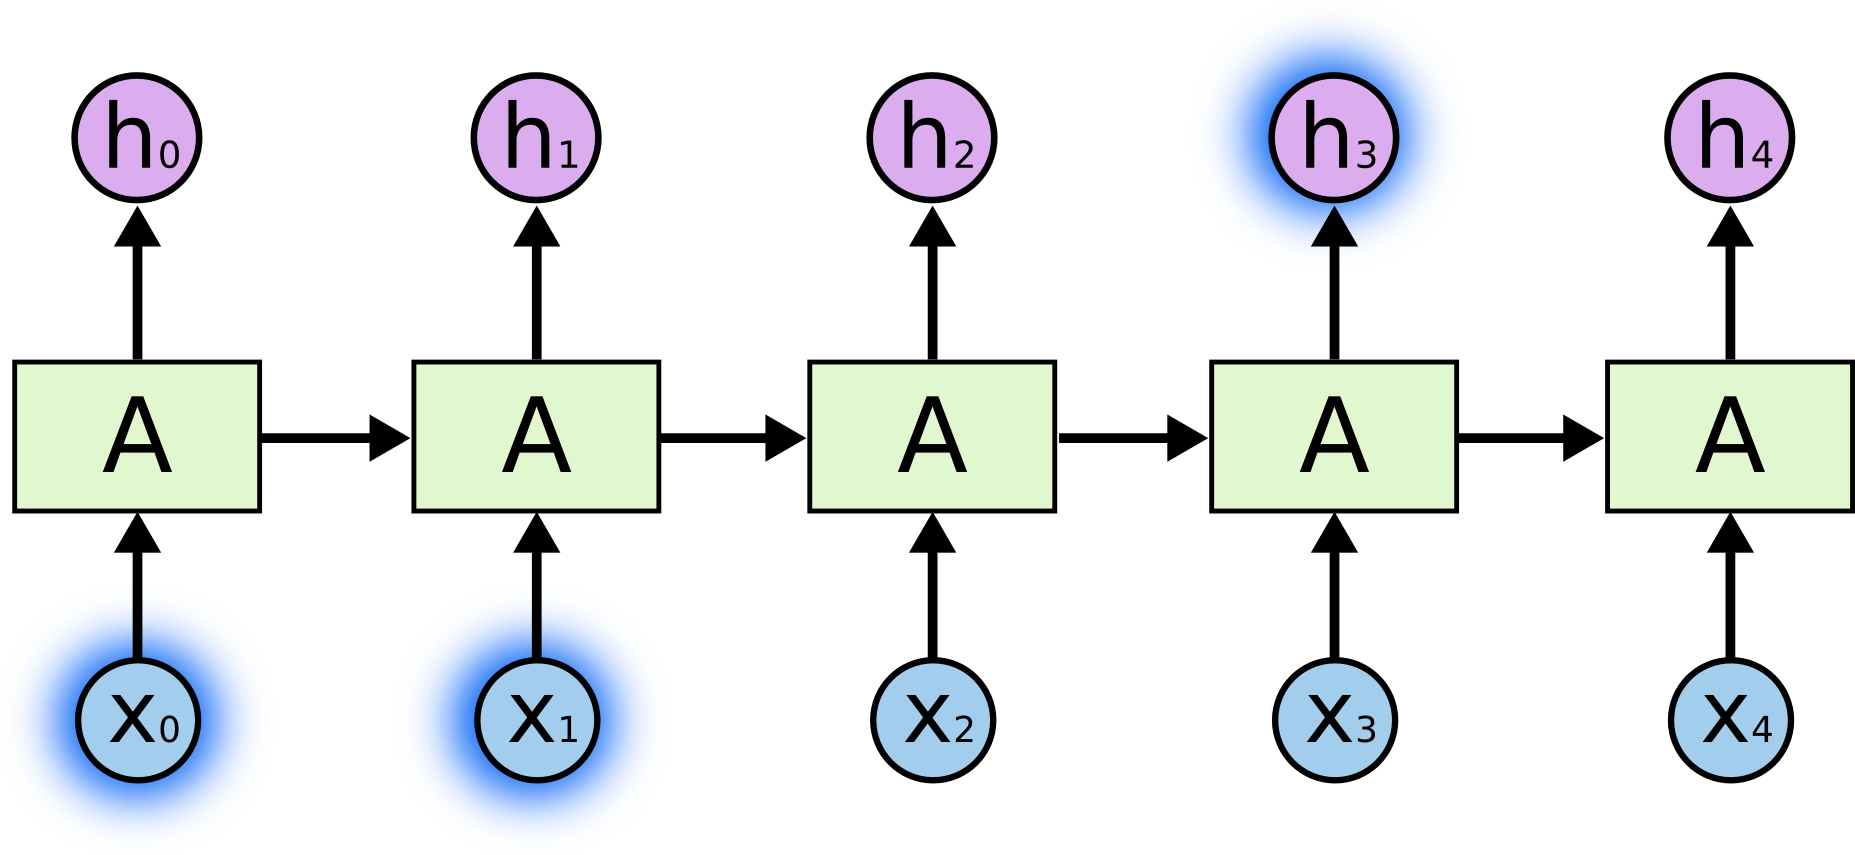
\includegraphics[width=\figureBigSize]
    {figure/model/RNN-shorttermdepdencies.png}}
\end{figure}

Nhưng cũng có những trường hợp chúng ta cần nhiều bối cảnh hơn. Cân nhắc việc cố gắng dự đoán từ cuối cùng trong văn
bản. "Tôi lớn lên ở Việt Nam. Tôi nói tiếng trôi chảy tiếng \textit{Việt}". Thông tin gần đây cho thấy từ tiếp theo có
lẽ là tên của một ngôn ngữ, nhưng nếu chúng ta muốn thu hẹp ngôn ngữ nào, chúng ta cần thu hẹp ngôn ngữ nào bối cảnh
của Việt Nam, từ phía trước. Nó hoàn toàn có thể cho khoảng cách giữa thông tin liên quan và điểm cần thiết để trở
nên rất lớn.

Thật không may, khi khoảng cách đó tăng lên, các RNN trở nên không thể học cách kết nối thông tin.
\begin{figure}[!htb]
    \center{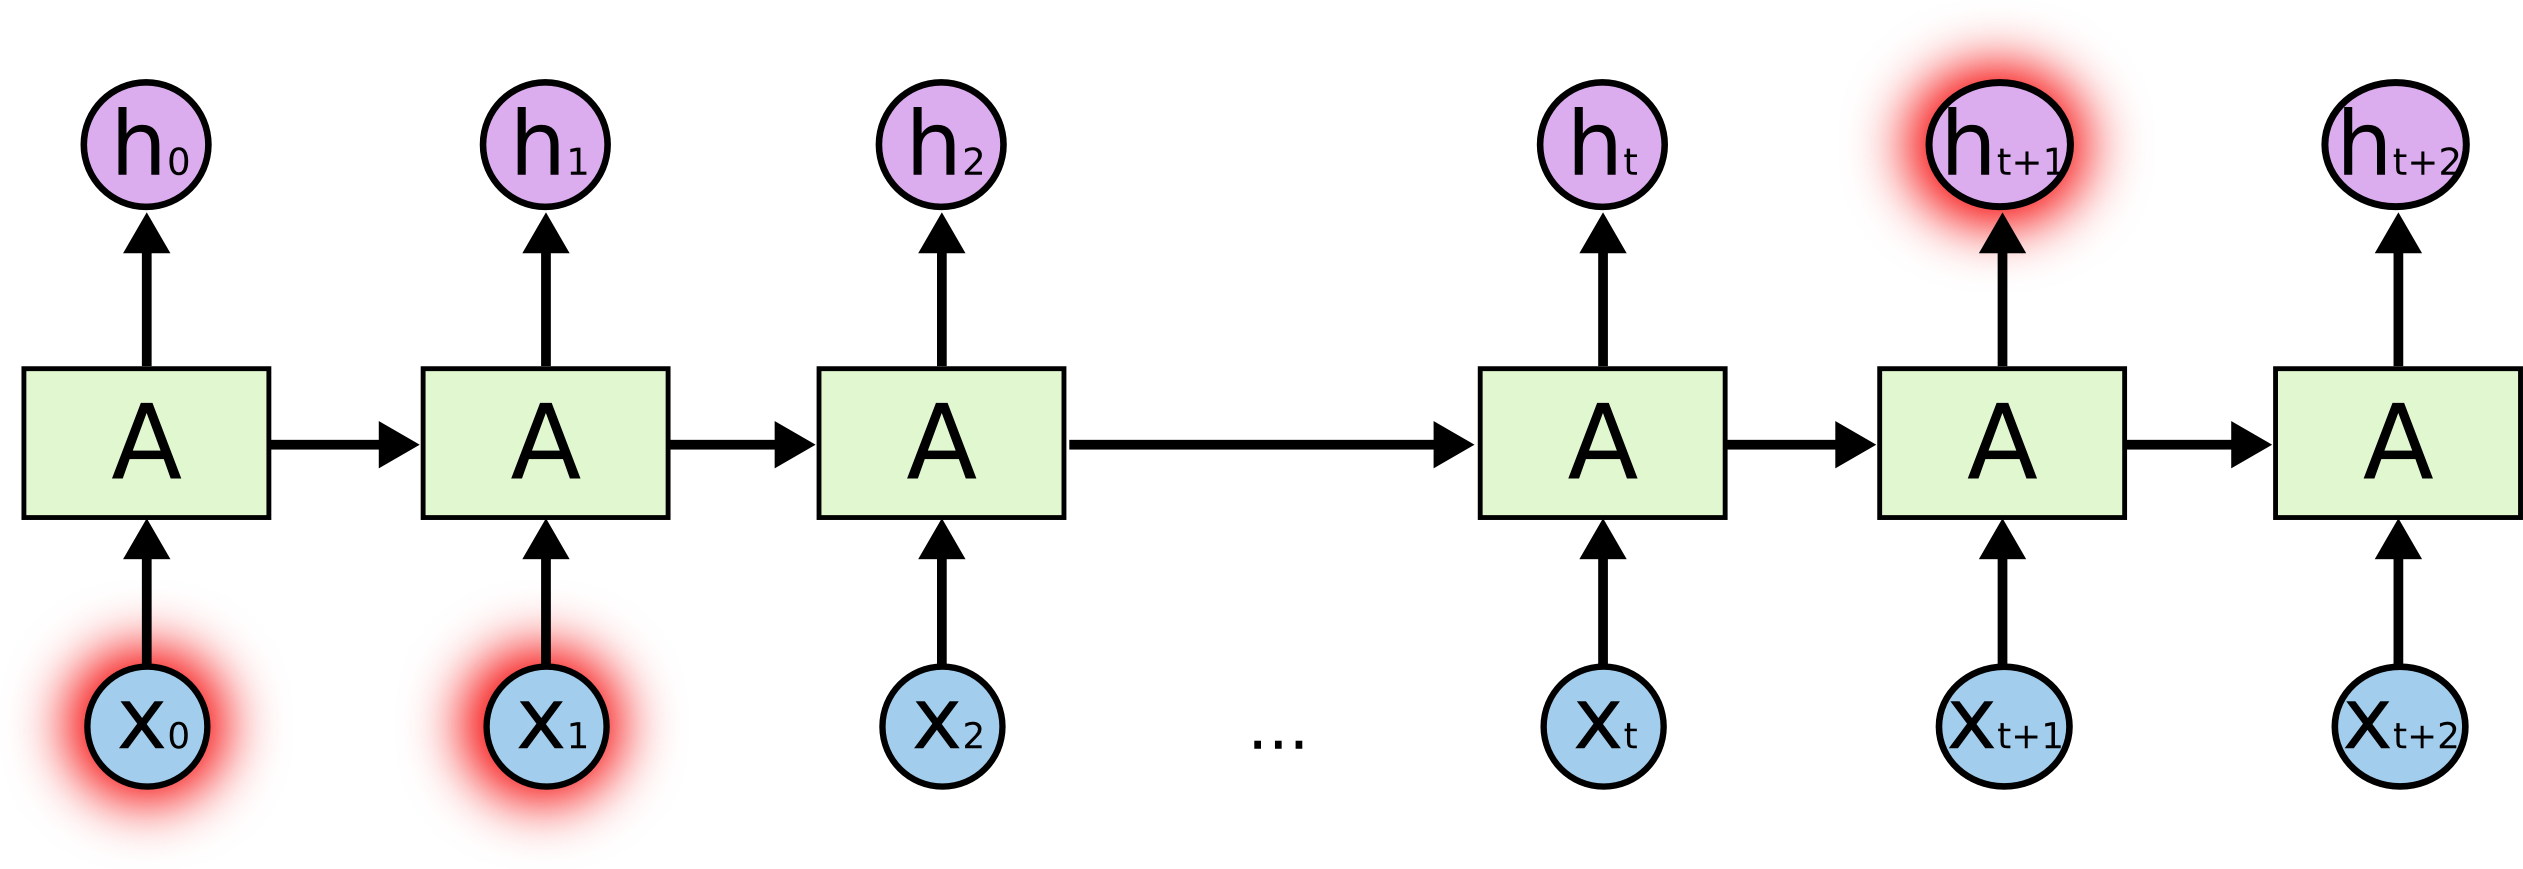
\includegraphics[width=\figureBigSize]
    {figure/model/RNN-longtermdependencies.png}}
\end{figure}


Về lý thuyết, các RNN hoàn toàn có khả năng xử lý các phụ thuộc dài hạn như vậy. Một người có thể cẩn thận chọn các
tham số cho họ để giải quyết các vấn đề về đồ chơi theo hình thức này. Đáng buồn thay, trong thực tế, RNNs don lồng
dường như có thể học chúng. Vấn đề đã được khám phá sâu bởi Hochreiter (1991) [German] và Bengio, et al. (1994),
người đã tìm thấy một số lý do khá cơ bản tại sao nó có thể khó khăn.

Rất may, LSTMs không có vấn đề này!

\textbf{Mạng LSTM} \\[0.2em]
Long Short Term Memory (mạng bộ nhớ dài ngắn hạn) - thường được gọi là LSTM của - - là một loại RNN đặc biệt, có khả năng học các phụ thuộc xa. Chúng được giới thiệu bởi Hochreiter \& Schmidhuber (1997), và được nhiều người tinh chỉnh và phổ biến. Chúng hoạt động rất tốt trong nhiều vấn đề lớn, và hiện đang được sử dụng rộng rãi.

Các LSTM được thiết kế rõ ràng để tránh vấn đề phụ thuộc dài hạn. Ghi nhớ thông tin trong thời gian dài thực tế là hành vi mặc định của nó, không phải là thứ khó khăn để học!

Tất cả các mạng thần kinh tái phát có dạng một chuỗi các module lặp lại của mạng thần kinh. Trong các RNN tiêu chuẩn, module lặp lại này sẽ có cấu trúc rất đơn giản, chẳng hạn như một lớp \(tanh\) duy nhất.

\begin{figure}[!htb]
    \center{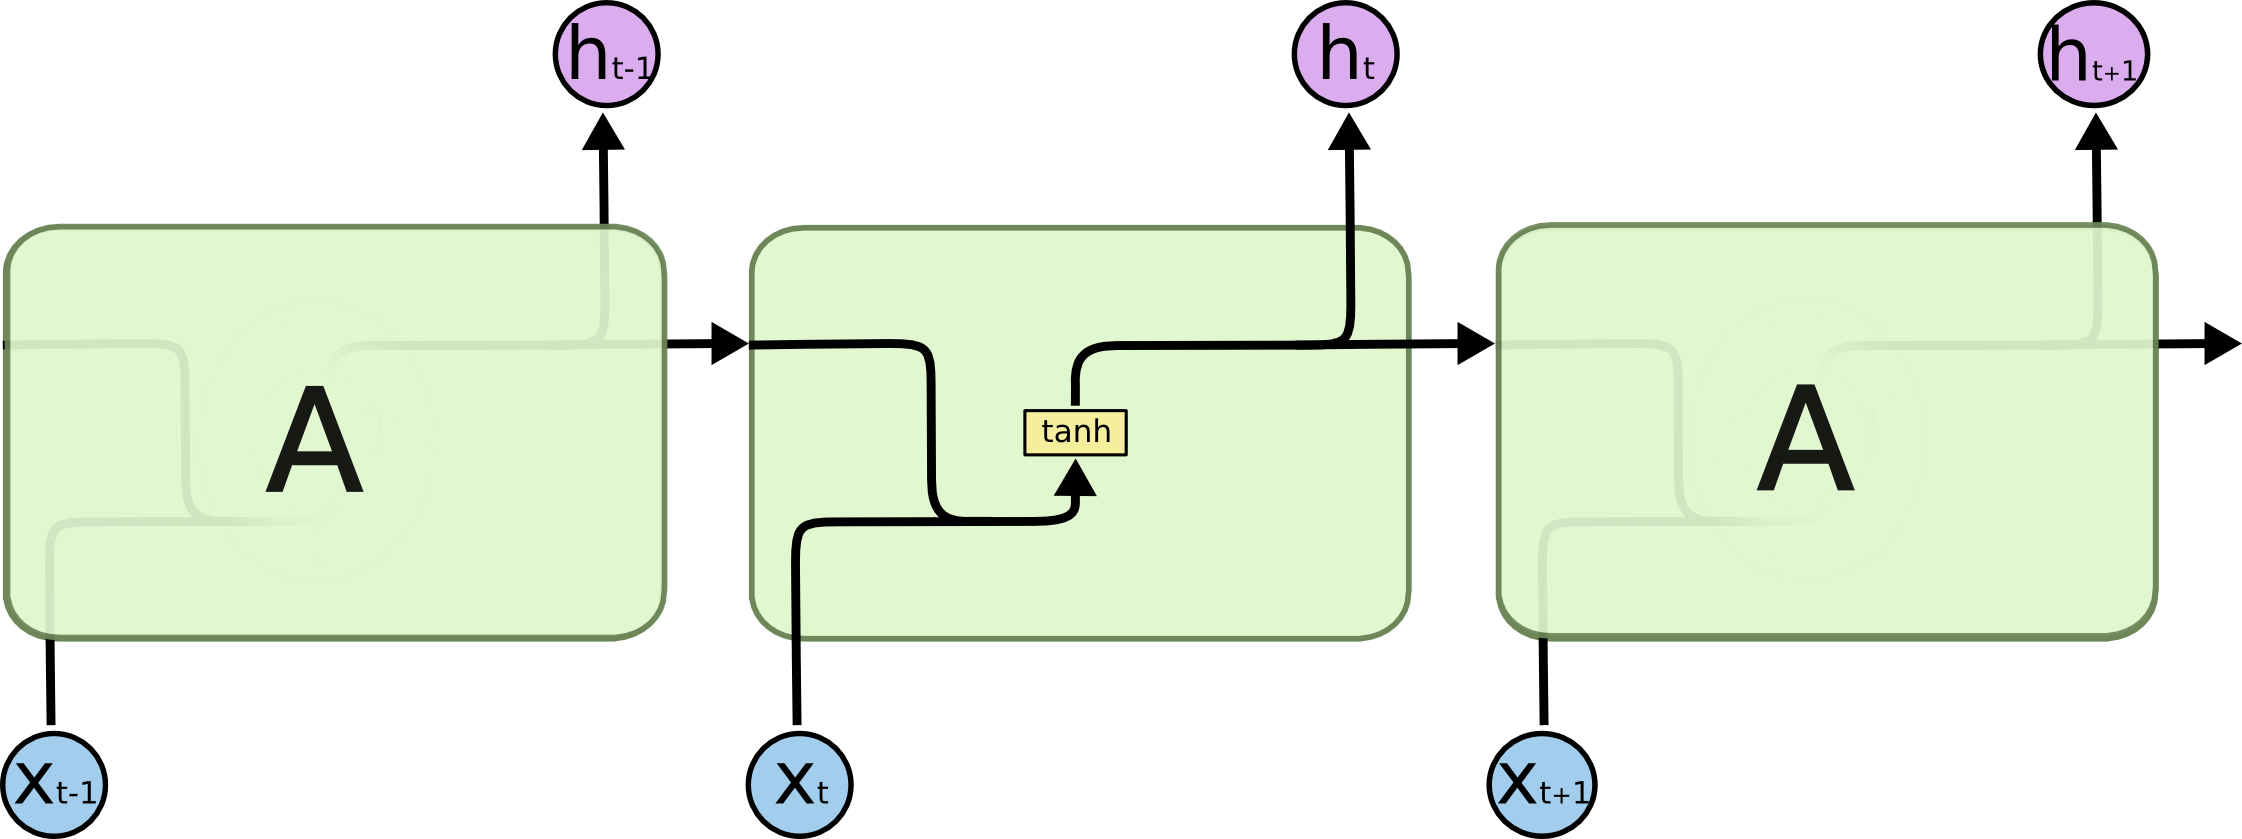
\includegraphics[width=\figureBigSize]
    {figure/model/LSTM3-SimpleRNN.png}}
    \caption{\label{fig:lstm3-simpleRNN} Module lặp trong RNN chuẩn chứa một lớp duy nhất.}
\end{figure}

LSTMs cũng có cấu trúc chuỗi, nhưng các module lặp có một cấu trúc khác. Thay vì có một lớp
mạng thần kinh duy nhất,nó có bốn lớp, tương tác theo một cách rất đặc biệt.

\begin{figure}[!htb]
    \center{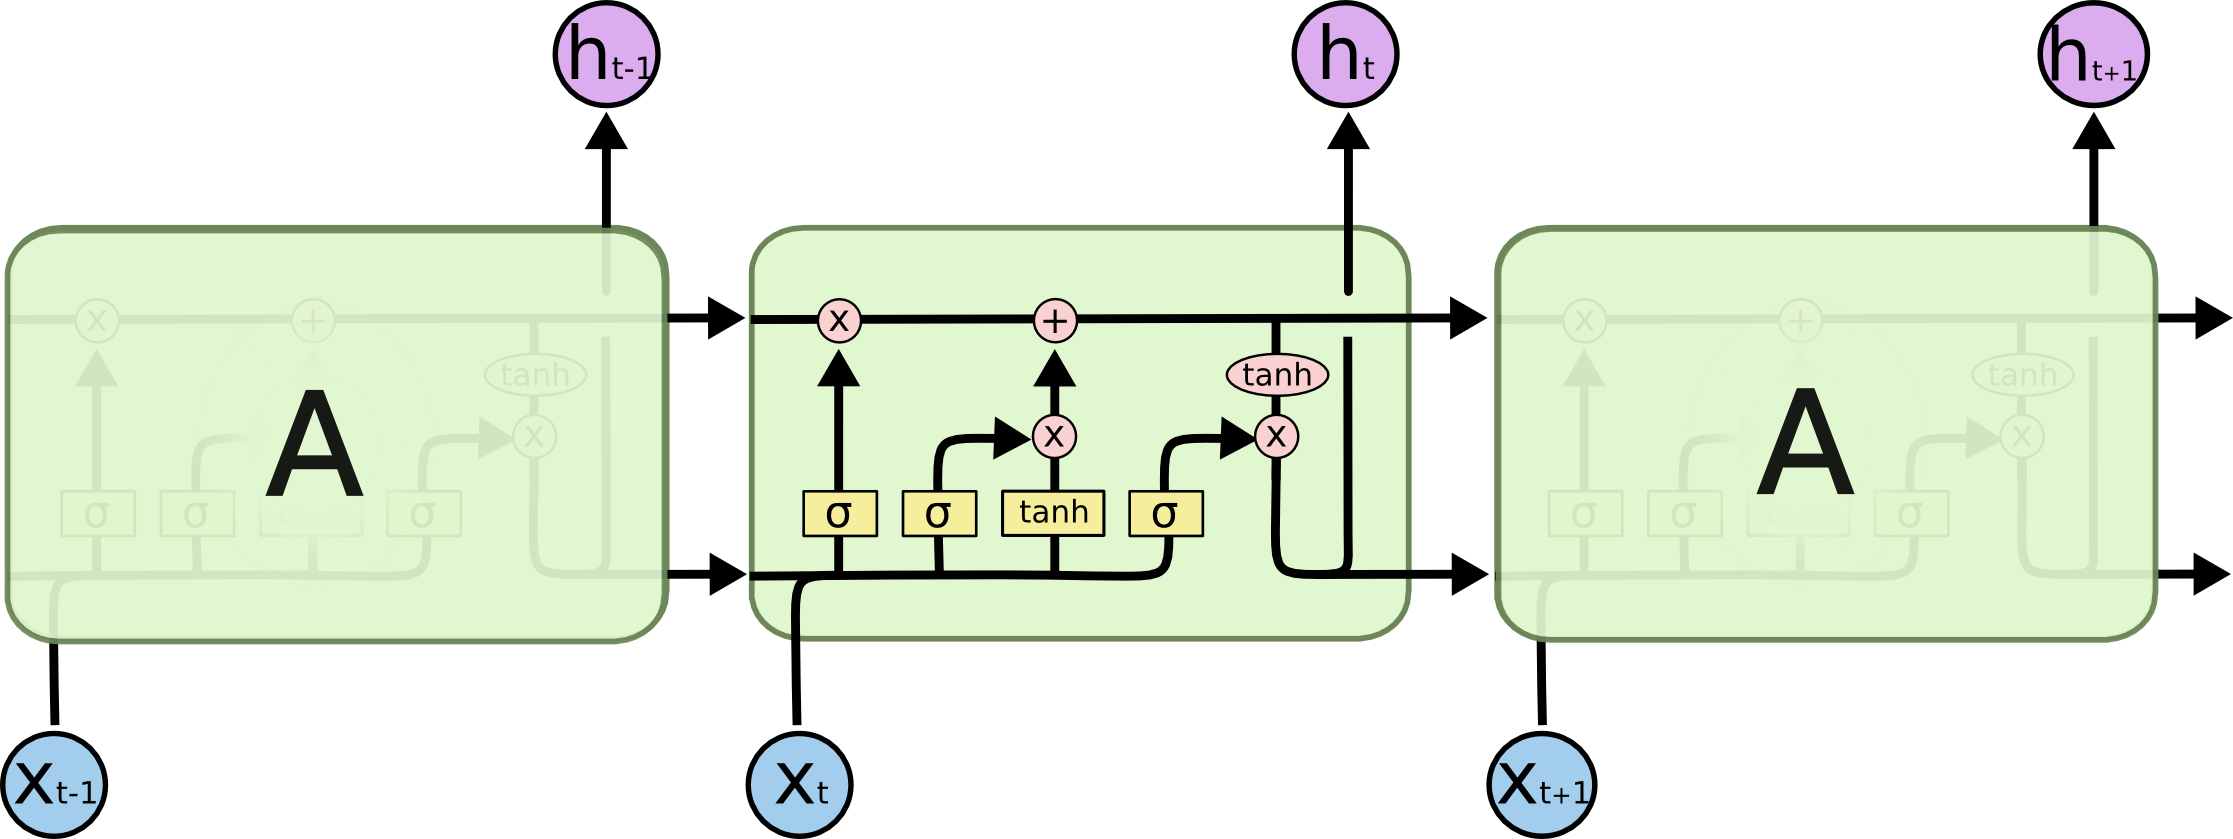
\includegraphics[width=\figureBigSize]
    {figure/model/LSTM3-chain.png}}
    \caption{\label{fig:lstm3-chain} Module lặp trong LSTM chứa 4 lớp tương tác.}
\end{figure}

\begin{figure}[!htb]
    \center{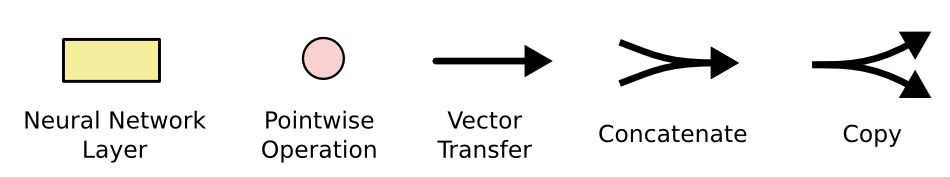
\includegraphics[width=\figureBigSize]
    {figure/model/LSTM2-notation.png}}
    \caption{\label{fig:lstm2-notation} Các ký hiệu trong LSTM.}
\end{figure}

Trong sơ đồ trên, mỗi dòng mang toàn bộ một vector, từ đầu ra của một nút đến đầu vào của các nút khác. Các vòng tròn
màu hồng đại diện cho các phép toán, như phép cộng vector, trong khi các hình chữ nhật màu vàng biểu thị các mạng
thần kinh để học. Các dòng hợp nhất biểu thị việc ghép nối, trong khi một dòng phân tách biểu thị nội dung của nó được
sao chép và các bản sao đi đến các vị trí khác nhau.

\textbf{Ý tưởng chính của LSTM} \\[0.2em]
Ý tưởng chính của LSTM là ô trạng thái, đường ngang chạy qua đỉnh sơ đồ.

Dòng trạng thái giống như một băng chuyền. Nó chạy thẳng xuống toàn bộ chuỗi, chỉ với một số tương tác tuyến tính nhỏ
dọc bên cạnh, dễ dàng cho thông tin truyền theo.

\begin{figure}[!htb]
    \center{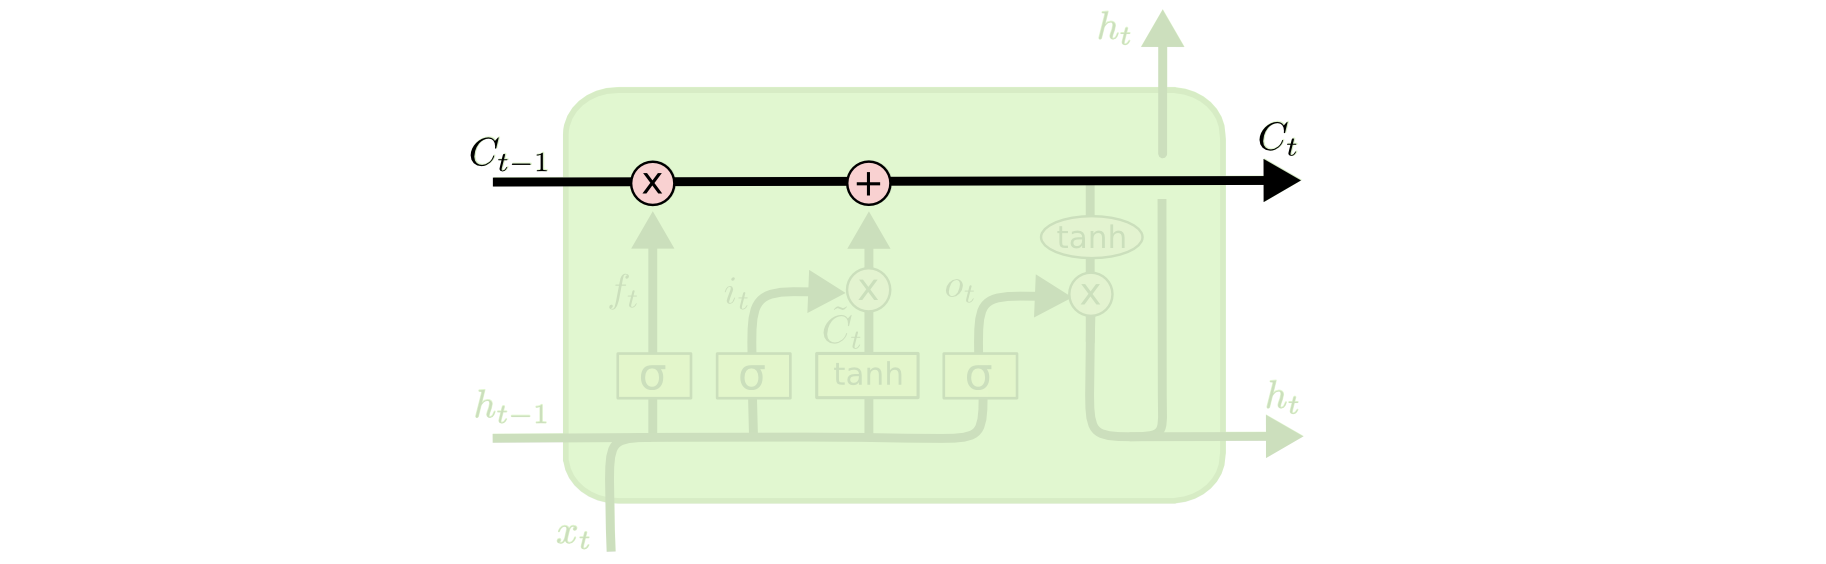
\includegraphics[width=\figureBigSize]
    {figure/model/LSTM3-C-line.png}}
\end{figure}

LSTM có khả năng loại bỏ hoặc thêm thông tin vào ô trạng thái, được điều chỉnh cẩn thận bởi các cấu trúc gọi là
cổng.

Cổng là một cấu trúc điều khiển thông tin thông qua. Chúng được cấu tạo từ một lớp lưới thần kinh \(sigmold\) và
một phép toán nhân.

\begin{figure}[!htb]
    \center{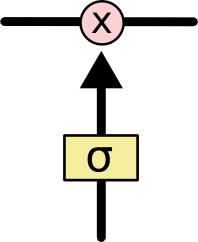
\includegraphics[width=1cm]
    {figure/model/LSTM3-gate.png}}
\end{figure}

Đầu ra của các lớp \(sigmoid\) có giá trị \([0, 1]\), mô tả mức độ cho qua. Giá
trị bằng \(0\) có nghĩa là không để bất cứ thứ gì qua, trong khi giá trị của \(1\) nghĩa
là có thể cho phép mọi thứ thông qua!

Một LSTM có ba trong cổng này, để bảo vệ và kiểm soát trạng thái tế bào.

\textbf{Các bước LSTM hoạt động} \\[0.2em]
Bước đầu tiên trong LSTM  là quyết định thông tin nào đi ra khỏi ô trạng thái. Quyết định này được đưa ra bởi
một lớp sigmoid được gọi là lớp "cổng quên". Nó dựa vào giá trị của \(h_{t-1}\) và \(x_t\), và đưa ra một số từ 0
đến 1 tương ứng với mỗi số ô trạng thái \(c_{t-1}\). Số 1 có nghĩa là giữ lại toàn bộ thông tin trong khi đó số 0 nghĩa
là hãy quên nó đi.

Hãy xem ví dụ của chúng ta về một mô hình ngôn ngữ đang cố gắng dự đoán từ tiếp theo dựa trên tất cả các từ trước đó.
Trong một vấn đề như vậy, ô trạng thái có thể bao gồm vai vế của ngữ hiện tại, để có thể sử dụng các động từ
một cách chính xác. Khi có một chủ ngữ mới, nó sẽ quên đi vai vế của chủ ngữ cũ.

\begin{figure}[!htb]
    \center{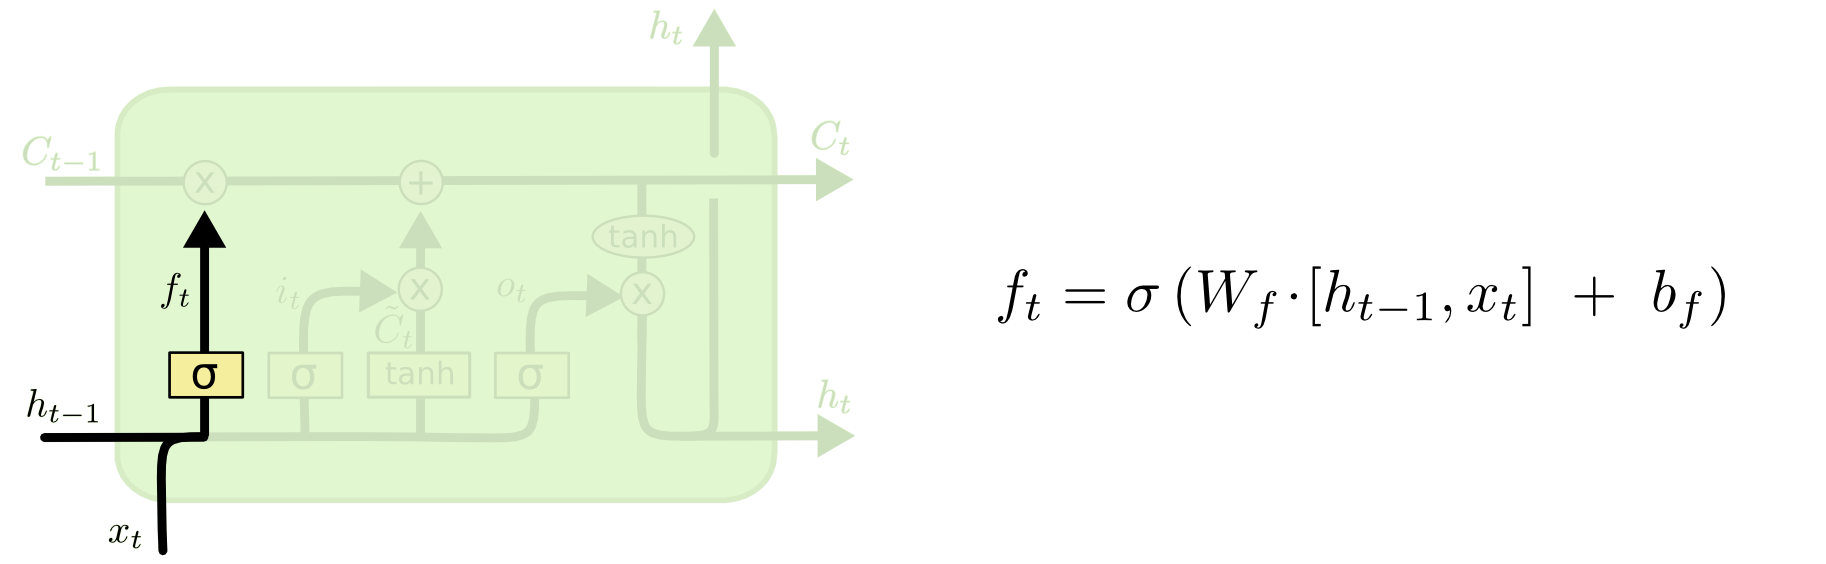
\includegraphics[width=\figureBigSize]
    {figure/model/LSTM3-focus-f.png}}
\end{figure}

Bước tiếp theo là quyết định những thông tin mới sẽ lưu trữ trong ô trạng thái. Việc này có hai phần. Đầu tiên,
một lớp sigmoid được gọi là lớp "cổng đầu vào" quyết định giá trị nào sẽ cập nhật. Tiếp theo, một lớp \(tanh\)
tạo ra một vector các giá trị ứng cử viên mới, \(C_t\), có thể được thêm vào ô trạng thái. Sau đó sẽ kết hợp  cả hai
để tạo ra một bản cập nhật cho trạng thái.

Trong ví dụ về mô hình ngôn ngữ, chúng tôi muốn thêm vai vế của chủ ngữ mới vào ô trạng thái, để thay thế chủ ngữ đã
quên.
\begin{figure}[!htb]
    \center{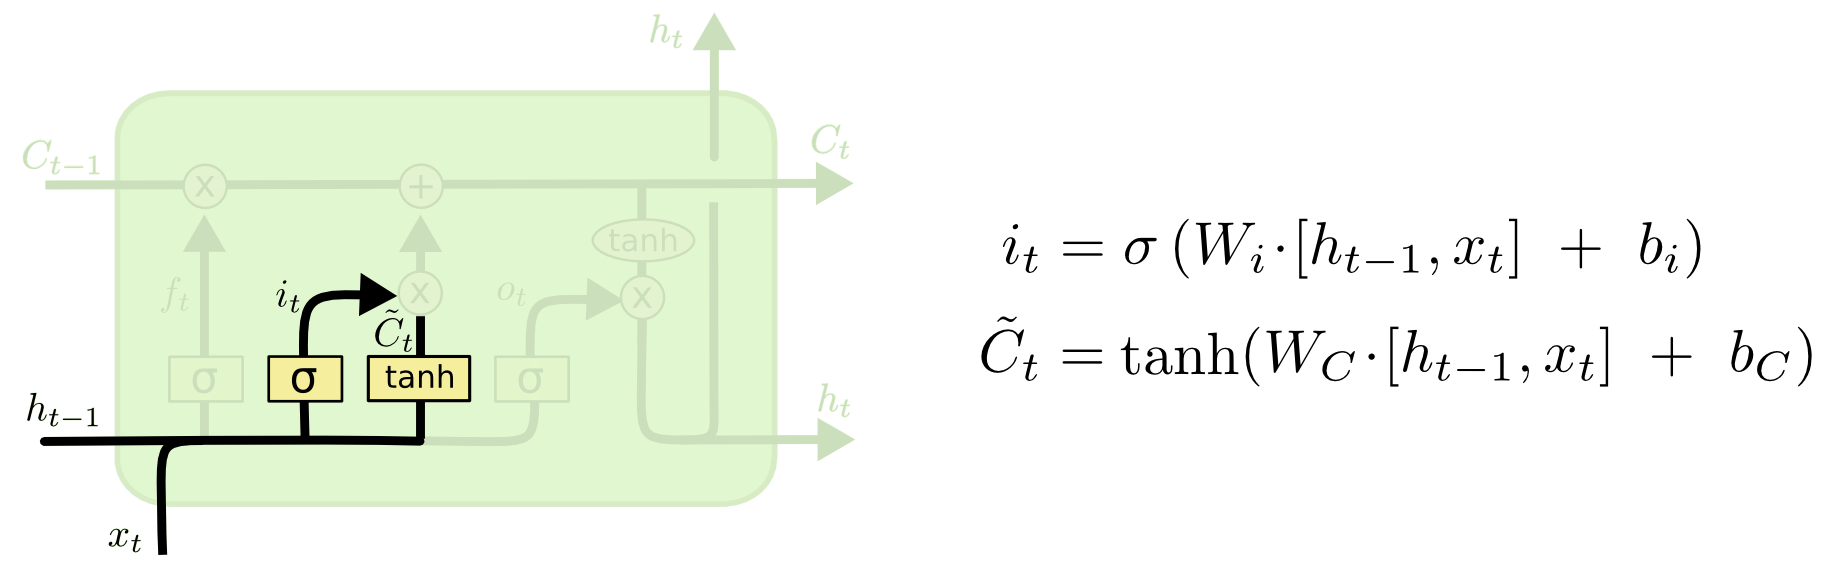
\includegraphics[width=\figureBigSize]
    {figure/model/LSTM3-focus-i.png}}
\end{figure}

Bây giờ, sẽ cập nhật ô trạng thái cũ, \(C_{t-1}\), sang ô trạng thái mới \(C_{t}\). Các bước trước đã quyết định phải
quên và nhớ những gì, giờ là lúc thực hiện nó.

Nhân ô trạng thái cũ với \(f_t\), quên đi những điều quyết định quên trước đó. Sau đó, cộng với \(i_t*\widetilde{C}_t\).
Đây là giá trị ứng viên mới, được tính theo mức độ cập nhật từng giá trị trạng thái.

Trong trường hợp của mô hình ngôn ngữ, đây là lúc thực sự bỏ thông tin về vai vế và thêm thông tin mới, như đã quyết
định trong các bước trước.
\begin{figure}[!htb]
    \center{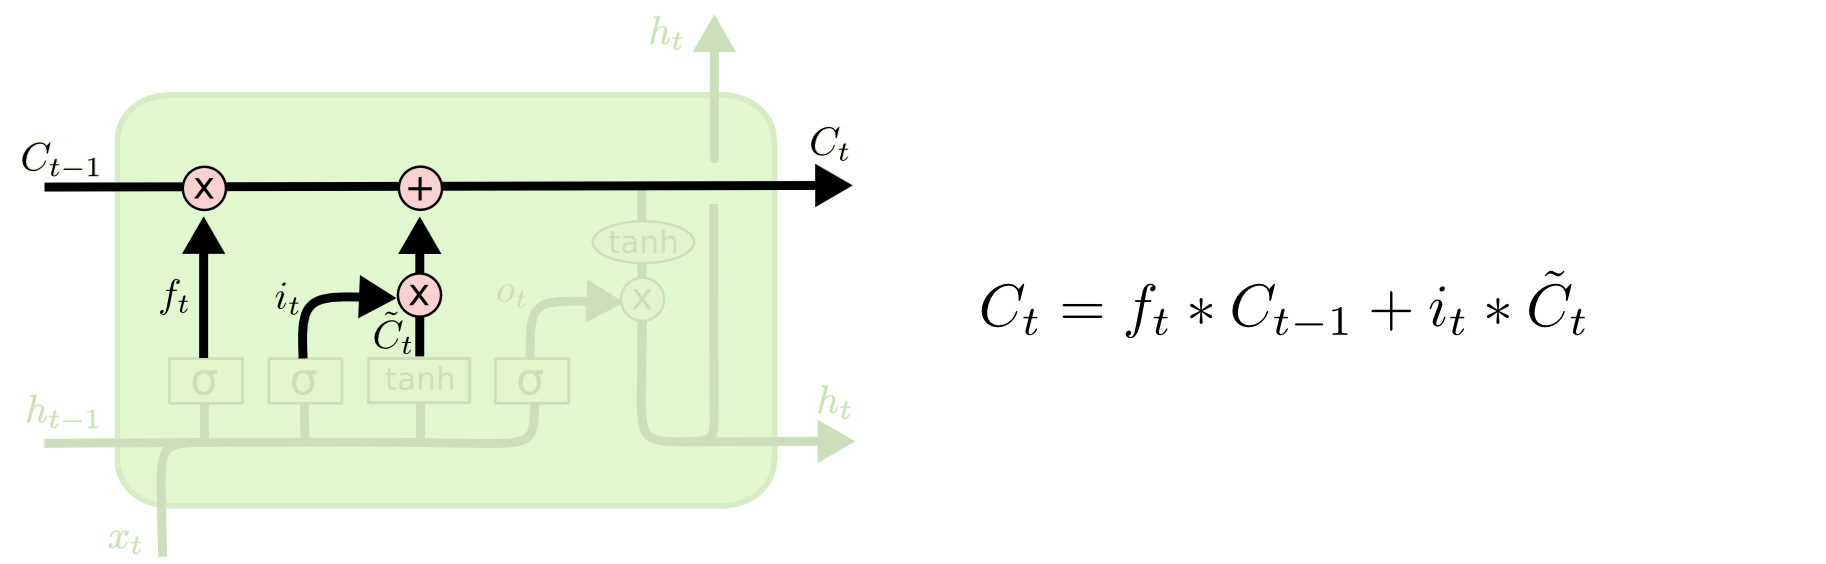
\includegraphics[width=\figureBigSize]
    {figure/model/LSTM3-focus-C.png}}
\end{figure}
Cuối cùng là quyết định những gì sẽ xuất ra. Đầu ra sẽ được lọc dựa vào ô trạng thái. Đầu tiên, chạy một lớp
\(sigmoid\) quyết định phần nào của ô trạng thái mà sẽ xuất ra. Sau đó, đưa ô trạng thái qua hàm
\(tanh\) (để đẩy các giá trị nằm trong khoảng -1 đến 1) và nhân nó với đầu ra của cổng \(sigmoid\), do đó chỉ đưa ra
các dữ liệu đã quyết định

Đối với ví dụ về mô hình ngôn ngữ, vì nó chỉ nhìn thấy một chủ ngữ, nó có thể muốn đưa ra thông tin có liên quan đến
một động từ, trong trường hợp đó là những gì sắp diễn ra. Ví dụ, nó có thể xuất ra vai vế của chủ ngữ , để biết được
cách dùng từ với chủ ngữ đó.

\textbf{Mạng GRU} \\[0.2em]
Ý tưởng của GRU cũng khá giống với LSTM:

\[ z = \sigma(x_t U^z + s_{t-1} W^z)  \]
\[r = \sigma(x_t U^r + s_{t-1} W^r)  \]
\[h = \tanh(x_t U^h + (s_{t-1} \circ r) W^h) \]
\[s_t = {(1 - z) \circ h} + {z \circ s_{t-1}} \]
​
GRU chỉ có 2 cổng: cổng thiết lập lại \(r\) và cổng cập nhập \(z\). Cổng thiết lập lại sẽ quyết định cách kết hợp giữa
đầu vào hiện tại với bộ nhớ trước, còn cổng cập nhập sẽ chỉ định có bao nhiêu thông tin về bộ nhớ trước nên giữa lại.
Như vậy RNN thuần cũng là một dạng đặc biệt của GRU, với đầu ra của cổng thiết lập lại là 1 và cổng cập nhập là 0.
Cùng chung ý tưởng sử dụng cơ chế cổng điều chỉnh thông tin, nhưng chúng khác nhau ở mấy điểm sau:
\begin{itemize}
    \item GRU có 2 cổng, còn LSTM có tới 3 cổng.
    \item GRU không có bộ nhớ trong \(c_t\) và không có cổng ra như LSTM.
    \item 2 cổng vào và cổng quên được kết hợp lại thành cổng cập nhập \(z\) và cổng thiết lập lại \(r\) sẽ được áp dụng trực tiếp cho trạng thái ẩn trước.
    \item GRU không sử dụng một hàm phi tuyến tính để tính đầu ra như LSTM.
\end{itemize}
\begin{figure}[!htb]
    \center{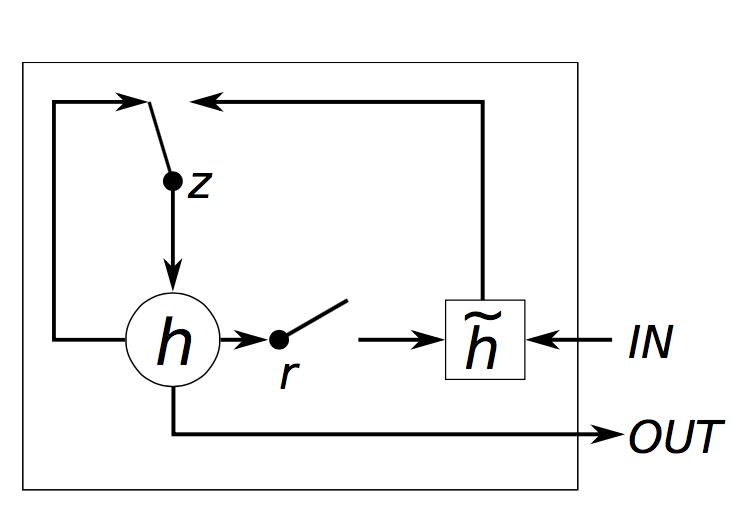
\includegraphics[width=\figureBigSize]
    {figure/model/GRU.png}}
    \caption{\label{fig:GRU} Các cổng GRU.}
\end{figure} % INCLUDE: introduction
    % !TEX root = ../chatbot-report.tex
%
\chapter{Tổng quan}
\label{sec:intro}

\section{Giới thiệu}
Dự đoán giá cổ phiếu là việc mà các nhà kinh tế thường xuyên bị hỏi.
Tuy nhiên việc dự đoán chính xác là một việc khó có thể làm vì có rất nhiều yếu tố ảnh hưởng.
Như cổ phiếu của một công ty chịu rất nhiều ảnh hưởng từ hoạt động công ty, chính phủ, quyết định của các nhà đầu tư.
Một số cá nhân, tổ chức có ảnh hưởng cực kì lớn tới giá cổ phiếu.
Với sự phát triển của internet thì thông tin được lan truyền rất nhanh, thông tin dường như gây ảnh hưởng đến giá cổ phiếu ngay lập tức

Đối với vàng thì thực sự không có một cá nhân tổ chức nào có thể nắm được quyền lực cụ thể.
Có rất nhiều nhân tố, một dòng twitter của tổng thống Mỹ Donald Trump không thể nào có những ảnh hưởng đáng kể tới giá vàng như việc tuyên bố cấm cửa Huawei của ông.

Thời trước đã có nhiều phương pháp để dự đoán giá vàng bằng phương pháp xây dựng mô hình thuần thống kê như
\begin{itemize}
    \item Autoregressive (AR)
    \item Moving Average (MA).
    \item Autoregressive Moving Average (ARMA)
    \item Autoregressive Integrated Moving Average (ARIMA)
    \item Seasonal Autoregressive Integrated Moving Average (SARIMA)
\end{itemize}
Những phương pháp này yêu cầu người dùng cần có rất nhiều kiến thức để tinh chỉnh tham số, đưa ra các dự đoán

Ngày nay, với sự phát triển của Machine Learning, có nhiều thuật toán mới tiến bộ, không yêu cầu người dùng phải
có kiến thực rộng lớn như cây quyết định, học sâu.

Trong cây quyết định có thuật toán nổi tiếng như XGBoost, LGB. Những thuật toán yêu cầu người dùng có khả năng đưa ra nhiều feature nhất có thể
để có thể đưa ra dự đoán chính xác

Học sâu có các mạng dòng họ Recurrent Neural Networks thường được sử dụng vì khả năng ghi nhớ thông tin trước đó. Phổ biến nhất là LSTM, GRU. Những thuật toán
này không cần người dùng đưa ra những feature nhưng những mạng này thường yêu cầu dữ liệu rất nhiệu và sức mạnh tính toán rất lớn để đưa ra dự đoán chính xác.

Gần đây, Facebook có đưa ra thuật toán Prophet. Sử dụng các tham số mặc định, Prophet đưa ra các dự đoán chính xác đánh ngạc nhiên mà không
tốn nhiều tài nguyên để tính toán.


\section{Đặt bài toán}
\label{sec:model:problem}
Bài toán đặt ra cho biết thông tin gía vàng trên sàng chứng khoáng hiện tại (GLD ETF). Làm sao để dự đoán 
được giá vàng đóng phiên của 90 ngày tiếp theo
Dự đoán được giá vàng sẽ giúp cho nhà đầu tư đưa ra được quyết định mua vào bán ra ngắn hạng, tạo điều kiện để
tích luỹ số tiền. Còn việc dự đoán xa hơn 90 ngày thì rất khó có thể chính xác và ít có ý nghĩa. Như lời khuyên từ Jack Welch cựu CEO cựu
General Electric, bạn nên để tất cả các trứng vào một giỏ và trông chừng nó. Hiếm có ai mà mua vàng để sinh lời mà lại không theo dõi giá cả hằng ngày.



\section{Xây dựng mô hình}
\label{sec:model:build}

\subsection{Dữ liệu}
Được lấy từ package python fix\_yahoo\_finance. Gói này lấy thông tin từ trang Yahoo Finance và chuyển thành Panda Dataframe.
Bảng này gồm 7 cột:
\begin{itemize}
    \item Date: ngày
    \item Open: giá lúc mở phiên
    \item Close: giá lúc đóng phiên
    \item High: giá cao nhất trong ngày
    \item Low: giá thấp nhất trong ngày
    \item Adj close: giá đóng phiên
    \item Volume: số lượng bán ra
\end{itemize}

\begin{table}[h]
	\begin{tabularx}{\textwidth}{X | X | X | X | X | X | X} 
		%\hline
		Date		& Open  & Date  & Close  & High  & Low & Adj close & Volume  		\\ \hline
		2004-11-18	& 44.43	& 44.490002000000004	& 44.07	 & 44.380001	& 44.380001	& 5992000		\\ %\hline
	\end{tabularx}
	\label{tab:table2}
	\caption{}
\end{table}

\begin{figure}[!htb]
    \center{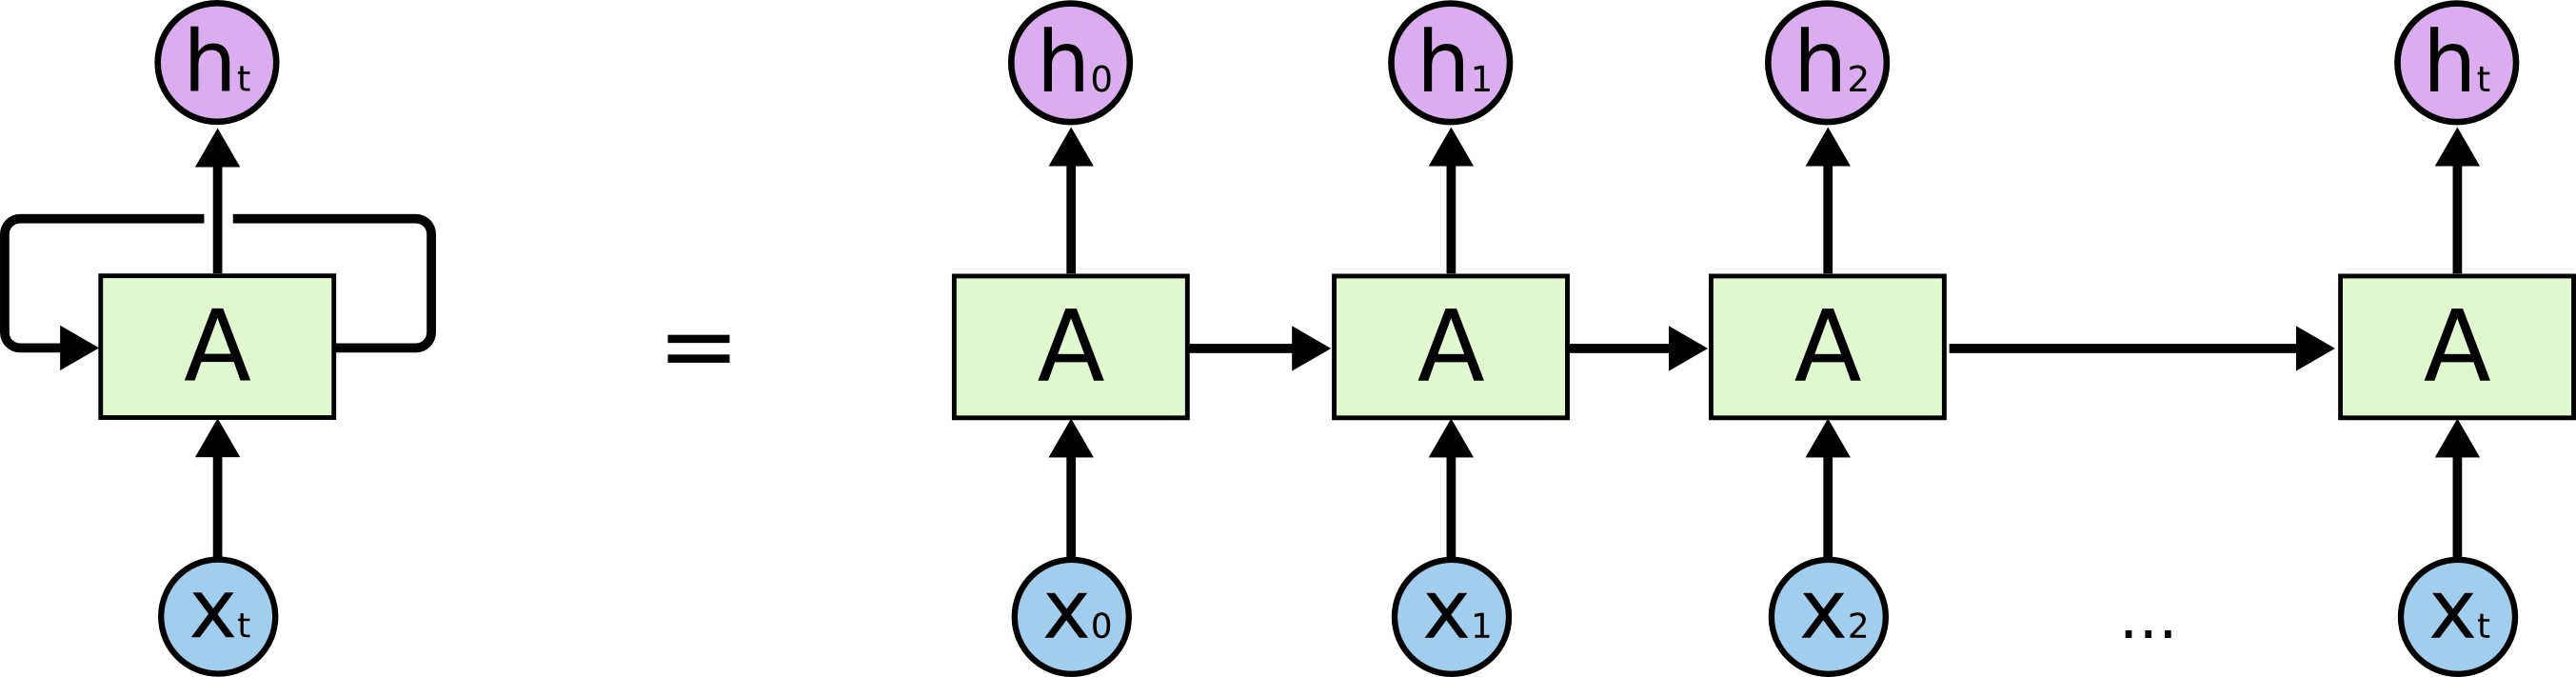
\includegraphics[width=\figureBigSize]
    {figure/model/RNN-unrolled.png}}
    \caption{\label{fig:gld-data} Biểu đồ dữ liệu}
\end{figure}

Dự liệu được lấy từ thị trướng chứng khoán, chính vì vậy, có những ngày nghỉ như ngày lễ, ngày thứ 7, chủ nhật sẽ không có dữ liệu.
Có vẻ như dữ liệu không có xu hướng trong năm, mùa và không bị ảnh hưởng bởi ngày lễ. Số lượng bán ra không phụ thuộc vào giá bán.

\subsection{Xử lý dữ liệu}

\textbf{Đối với mạng học sâu}
Chuyển thành bài toán học có giám sát
\begin{itemize}
    \item Đối với những ngày không có dữ liệu thì điền dữ liệu bằng ngày trước để có tính liên tục \\
    \item Giữ lại cột: Date, Close. Đổi tên cột Date thành ds, Close thành y. Bỏ các cột còn lại(Theo quy chuẩn) \\
    \item Chuẩn hoá dữ liệu cột y bằng MinMaxScalar với khoảng (0, 1) \\
    \item Giữ 90 ngày cuối để xác minh. Những ngaỳ còn lại để đem train \\
    \item Dữ liệu đầu vào: sẽ ra giá của 90 ngày trước ngày hiện tại \\
    Dữ liệu đầu ra là giá vàng của ngày hiện tại +  89 ngày sau ngày hiện tại. Vậy sẽ bỏ qua 90 ngày đầu của bộ dữ liệu (thiếu dữ liệu ngày trước đó). 90 ngày cuối vẫn giữ lại. Đối với những ngày không có dữ liệu thì điền vào 0 \\
\end{itemize}
\begin{table}[h]
	\begin{tabularx}{\textwidth}{X | X | X | X | X | X | X} 
		%\hline
		y\_past\_1	& y\_past\_2	 & y\_past\_3	& ...	& y\_past\_88	 & y\_past\_89	 & y\_past\_90 		\\ \hline
		0.009210	& 0.009000	& 0.005721	& ... & 0.024559	& 0.024559	& 0.021768\\ \hline
		...	& ...	& ...	& ... & ...	& ...	& ...\\ \hline
		0.512300	& 0.540010	& 0.531230	& ... & 0.550120	& 0.550300	& 0.550309\\ %\hline
	\end{tabularx}
	\label{tab:table2}
	\caption{Dữ liệu đầu vào mẫu}
\end{table}
\begin{table}[h]
	\begin{tabularx}{\textwidth}{X | X | X | X | X | X | X} 
		%\hline
		y	& y\_future\_1 & y\_future\_2	& ...	& y\_future\_87	 & y\_future\_88	 & y\_future\_89		\\ \hline
		0.008791	& 0.010256	& 0.010396		& ... & 0.004814	& 0.004814	& 0.004326\\ \hline
		...	& ...	& ...		& ... & ...	& ...	& ...\ \hline
		0.520001	& 0	& 0		& ... & 0	& 0	& 0\\ %\hline
	\end{tabularx}
	\label{tab:table2}
	\caption{Dữ liệu đầu vào ra}
\end{table}

\textbf{Đối với Prophet}
Chuyển thành bài toán học có giám sát
\begin{itemize}
    \item Đối với những ngày không có dữ liệu thì điền dữ liệu bằng ngày trước để có tính liên tục \\
    \item Giữ lại cột: Date, Close. Đổi tên cột Date thành ds, Close thành y. Bỏ các cột còn lại(Theo quy chuẩn) \\
    \item Giữ 90 ngày cuối để xác minh. Những ngày còn lại để đem train \\
\end{itemize}
\begin{table}[h]
	\begin{tabularx}{\textwidth}{X | X | X | X | X | X | X} 
		%\hline
		ds	& y	  \\ \hline
		2019-03-01	& 121.879997 \\ \hline
		2019-03-02	& 121.879997 \\ \hline
		2019-03-03	& 121.879997 \\ \hline
		2019-03-04	& 121.879997 \\ \hline
		2019-03-05	& 121.879997 \\ %\hline
	\end{tabularx}
	\label{tab:data_prophet}
	\caption{Dữ liệu mẫu Prophet}
\end{table}







 % INCLUDE: data work
    \chapter{Những đóng góp của nhóm}
\label{sec:contribute}
\begin{enumerate}
    \item Thay đổi phương pháp chuẩn hoá, loss function
    \item Đề xuất công thức để đánh giá mô hình
    \item Bổ sung mạng đơn giản đê tăng độ chính xác
    \item Thêm các biểu đồ trực quan
    \item Bổ sung mô hinh Facebook Prophet
\end{enumerate}

    % --------------------------
    % Back matter
    % --------------------------
    {%
    	\setstretch{1.1}
    	\renewcommand{\bibfont}{\normalfont\small}
    	\setlength{\biblabelsep}{0pt}
    	\setlength{\bibitemsep}{0.5\baselineskip plus 0.5\baselineskip}
        \nocite{*}
        \printbibliography[title={Tài liệu tham khảo}]
        \cleardoublepage
%    	\printbibliography[heading=subbibliography,title={Website},type=online,prefixnumbers={@}]
    }

    \newpage
    \mbox{}

    % **************************************************
    % End of Document CONTENT
    % **************************************************
\end{document}
